\chapter{On-Chain Design}
\label{chap:onchainDesign}
This chapter details the on-chain design of the \acrshort{ew} system, which is implemented entirely via smart contracts. As introduced previously, these contracts embody the core logic of the platform, exposing the functionality required by both the \acrshort{sdk} and the browser extension. Their overall structure is depicted in the class diagram in \cref{fig:contractsClass}. 

The \acrshort{ew} system comprises seven custom smart contracts, represented as white classes in the diagram. (\textit{Result} is not a smart contract, see \cref{sec:studentContract} for more details). 
\begin{enumerate}
    \item \textbf{SmartAccount}: Defines the structure of a \acrfull{sca} following the account abstraction specification.
    \item \textbf{Student}: Represents an individual student in the system.
    \item \textbf{University}: Represents a university entity.
    \item \textbf{StudentDeployer}: Responsible for deploying Student contracts.
    \item \textbf{UniversityDeployer}: Deploys University contracts.
    \item \textbf{StudentsRegister}: Manages and stores information about students and universities.
    \item \textbf{Paymaster}: Sponsors blockchain transactions made by students and universities.
\end{enumerate}
It addition, the system relies on five external contracts, shown in green in \cref{fig:contractsClass}, which are derived from established libraries such as \textit{OpenZeppelin}:
\begin{enumerate}
    \item \textbf{EntryPoint}: A contract that receives transactions from smart accounts and executes user operations.
    \item \textbf{AccessControl}\footnote{\url{https://docs.openzeppelin.com/contracts/5.x/api/access}}: Provides a comprehensive role-based access control mechanism.
    \item \textbf{Ownable}\footnote{\url{https://docs.openzeppelin.com/contracts/5.x/api/access\#Ownable}}: Implements a simple ownership model, allowing the designated owner to perform privileged operations via restricted functions.
    \item \textbf{BaseAccount}: Abstract contract defining the core behaviours of a \acrshort{sca} under the account abstraction specification.
    \item \textbf{BasePaymaster}: Abstract contract defining the structure of a paymaster that sponsors user transactions.
\end{enumerate}

Before detailing the design of each custom smart contract and its role in the academic records workflow, we first justify our choice on on-chain technologies and platforms. 

\begin{figure}
  \centering
  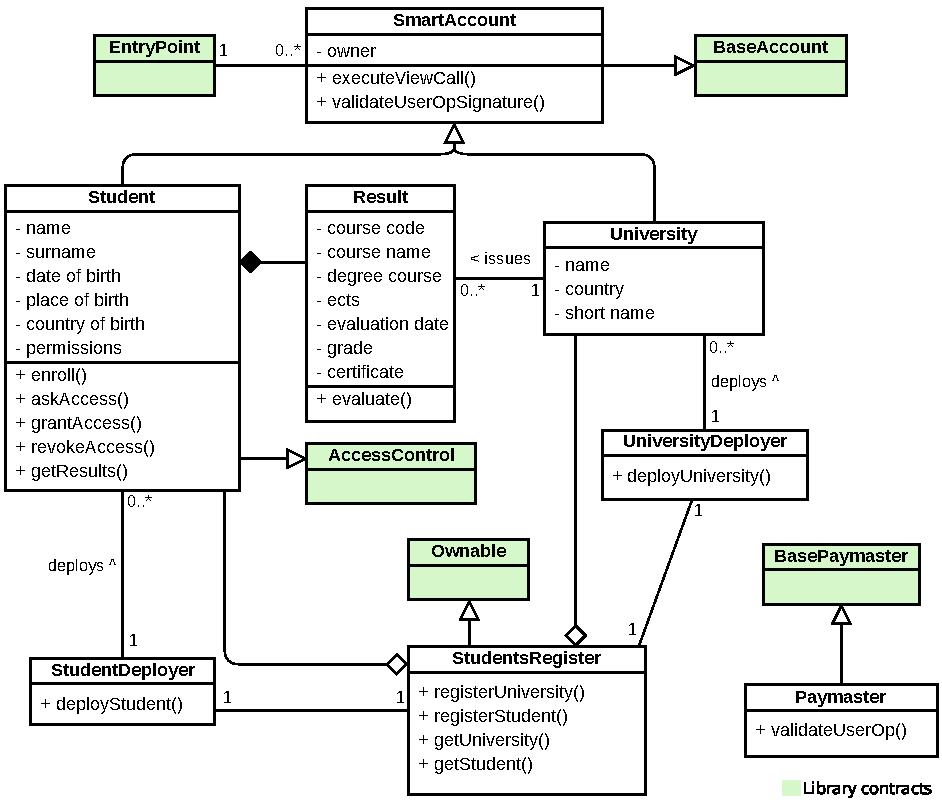
\includegraphics[width=1\textwidth]{figures/Contracts class diagram.pdf}
  \caption[Smart contracts architecture class diagram]{Class diagram representing smart contracts architecture}
  \label{fig:contractsClass}
\end{figure}

%%%%%%%%%%%%%%%%%%%%%%%%%%%%%%%%%%%%%%%%%%%%%%%%%%%%%%%%%%%%%%%%%%
% BLOCKCHAIN TECHNOLOGIES
%%%%%%%%%%%%%%%%%%%%%%%%%%%%%%%%%%%%%%%%%%%%%%%%%%%%%%%%%%%%%%%%%%
\section{Blockchain Technologies}
The development of a blockchain-based system begins with the selections of a suitable blockchain platform. We selected \acrlong{eth}, a public blockchain known for its extensive developer community and rich ecosystem of features particularly suitable for an academic record systems \cite{mustafa2024publiceduchain}\cite{yassynzhanbolatzhan2021verificationuniversitystudent}. \acrlong{eth} supports smart contract development in multiple languages and serves as the foundation for various layer 2 solutions that enhance performance and scalability\cite{sguanci2021layer2blockchainscaling}. This flexibility allows the system to be initially developed for the \acrlong{eth} mainnet and later migrated to a layer 2 chain to take advantage of specific features, with minimal development overhead. 

For the implementation, we selected Solidity\footnote{\url{https://soliditylang.org/}} as the programming language. Solidity is an object-oriented language, designed specifically for writing smart contracts on \acrlong{eth} and the \acrshort{evm}, influenced by C++, JavaScript and Python\footnote{\url{https://github.com/ethereum/solidity/blob/develop/docs/index.rst}}. It is the most widely adopted language in the \acrlong{eth} ecosystem, supported by and active and large developer community. Given our prior experience with Solidity, this choice was natural and well-suited to our objectives.

\subsection{Account Abstraction}
\label{ssec:accountAbstraction}
One of the most significant obstacles to the widespread adoption of blockchain technologies, and Web3 applications in general, is the complexity involved in interacting with the blockchain. To perform on-chain operations, users are typically required to create and manage cryptocurrencies wallets (\acrfull{eoa}), fund them with tokens (e.g., Bitcoin or \acrlong{eth}), and only then are they able to access and utilize decentralized platforms. During the design of the system, we aimed to eliminate this burden for users, in order to streamline the interactions among \acrlong{ew}, universities and students, thereby addressing \acrshort{nfr} 5 in \cref{tab:nonFuncReq}. These considerations motivated the adoption of account abstraction within the system.

\begin{figure}
  \centering
  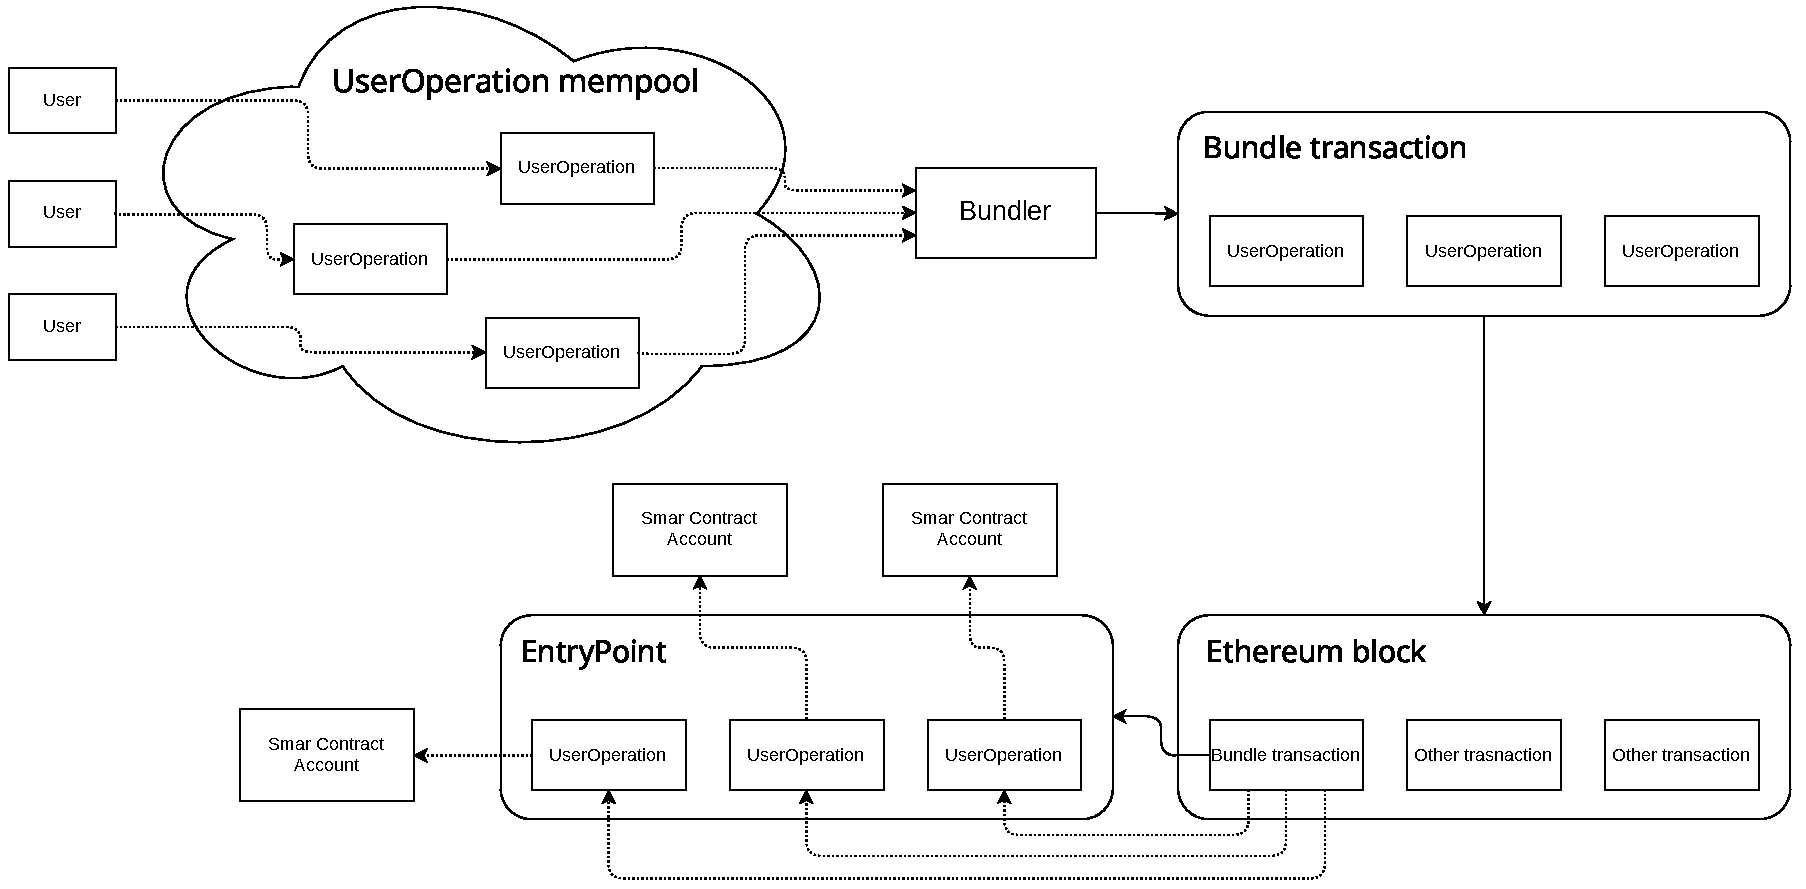
\includegraphics[width=1\textwidth]{figures/Account Abstraction.pdf}
  \caption[UserOperation life cycle within account abstraction protocol]{UserOperation life cycle within account abstraction protocol.}
  \label{fig:accountAbstraction}
\end{figure}

ERC‑4337, introduced in September 2021 by Vitalik Buterin and others\cite{buterin2021erc}, defines account abstraction on Ethereum. It enables users to leverage \acrlong{sca} with custom logic as their primary on‑chain accounts, replacing traditional \acrshort{eoa}. User actions are encapsulated in pseudo‑transactions called \textit{UserOperations}, whose life cycle is illustrated in \cref{fig:accountAbstraction}. Each UserOperation may bundle multiple on‑chain actions, such as contract calls or token transfers, and includes all necessary execution data. When creating a UserOperation, the user specifies the target \acrshort{sca} and signs the operation to authorize both its execution and associated gas consumption.
Signed UserOperations are submitted to a \gls{mempool}, where specialized nodes called bundlers collect and aggregate them into a single on‑chain transaction. This transaction is sent to an entry point contract on Ethereum, which unpacks each UserOperation and dispatches it to the designated \acrshort{sca}. The \acrlong{sca} then executes the required actions and handles fee payments, effectively becoming the transaction sender.

A key feature of ERC‑4337 is the ability to designate a paymaster, such as our system’s Paymaster contract, to sponsor gas fees on the user’s behalf. If the paymaster approves, it covers the transaction costs, allowing users to interact with \acrlong{ew} without managing wallets or tokens directly.

This standard also introduces in \acrlong{eth} several notable features:
\begin{itemize}
    \item \textbf{Custom Verification Logic}: \acrlong{sca}s have the capacity to implement custom-made authentication and validation mechanisms, going beyond the traditional public-key signature model.
    \item \textbf{Sponsored Transactions}: Developers can delegate gas payment to paymaster, transforming the user fee experience.
    \item \textbf{Bundled Operations}: Users can combine multiple transactions into a single UserOperation, reducing the aggregate cost compared to separate transactions.
\end{itemize}

In our local test environment, where no public bundler is available, UserOperations are sent directly to the entry point contract, which then forwards them to the corresponding \acrshort{sca} for execution.

%%%%%%%%%%%%%%%%%%%%%%%%%%%%%%%%%%%%%%%%%%%%%%%%%%%%%%%%%%%%%%%%%%
% SMART ACCOUNT
%%%%%%%%%%%%%%%%%%%%%%%%%%%%%%%%%%%%%%%%%%%%%%%%%%%%%%%%%%%%%%%%%%
\section{SmartAccount}
\label{sec:smartAccountDesign}
Depicted in \cref{fig:smartAccountContractClass}, \textit{SmartAccount} contract serves as an abstract base for all \acrlong{sca}s in the account-abstraction layer of the \acrlong{ew} system. Both University and Student contracts inherit from SmartAccount, which in turn extends BaseAccount, an abstract contract supplied by the ERC-4337 standard. BaseAccount implements core ERC-4337 logic, including support for both single and batched UserOperations and a mechanism to refund the entry point contract for gas expenditures incurred during transaction execution.

\begin{figure}
  \centering
  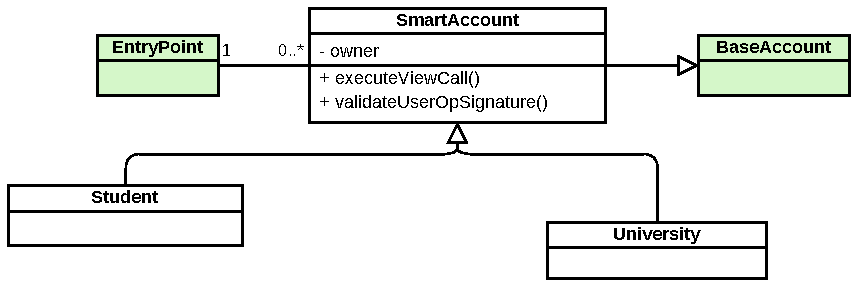
\includegraphics[width=0.7\textwidth]{figures/SmartAccount class diagram.pdf}
  \caption[Class diagram focused on SmartAccount contract]{Class diagram showing a focused view of the SmartAccount contract and its associated interactions. This view is a subset of the broader system architecture.}
  \label{fig:smartAccountContractClass}
\end{figure}

SmartAccount boosts these capabilities with two key features:
\begin{itemize}
    \item \textbf{Validate UserOperation Signature}: Upon receiving a signed UserOperation, the contract verifies that the signature originates from owner of the \acrshort{sca}. The owner is specified when the contract which implements SmartAccount is deployed by providing the address to its constructor. Once validated, the account can perform the specified operations by leveraging the execution routines provided BaseAccount.
    \item \textbf{Execute Read-Only Function}: To allow gasless access to read-only (\textit{view}) functions that are permissioned in our system, the contract offers a dedicated method, restricted to only the owner of the account, for executing such calls via the \acrshort{sca}. This avoids the need for standard UserOperations execution, and their associated gas costs, when users only require data retrieval. These view calls are performed by providing SmartAccount the address of the target contract and the encoded function data (\textit{calldata}) to send to it (i.e., the function signature and parameters in encoded form).
\end{itemize}

Moreover, because \acrlong{sca}s support customizable signature validation logic and decouple externally \acrshort{eoa}s from on-chain execution, SmartAccount can be readily adapted to integrate alternative authentication schemes.

%%%%%%%%%%%%%%%%%%%%%%%%%%%%%%%%%%%%%%%%%%%%%%%%%%%%%%%%%%%%%%%%%%
% STUDENT
%%%%%%%%%%%%%%%%%%%%%%%%%%%%%%%%%%%%%%%%%%%%%%%%%%%%%%%%%%%%%%%%%%
\section{Student}
\label{sec:studentContract}
The \textit{Student} contract encapsulates the majority of the system's logic. Its primary responsibilities include storing the student's personal information, such as name, surname, date of birth, place of birth and country of birth, as well as managing their academic records. These records are stored using the structure presented in \cref{lst:resultStruct}. 
\lstinputlisting[
    caption={\textit{Result} structure within the \textit{Student} smart contract},
    label=lst:resultStruct,
    language=Solidity,
]{listings/result.sol}
Due to Solidity's limited support for floating-point numbers, and because the \acrshort{ects} credits may not always be whole number, the \acrshort{ects} value is stored as the original number multiplied by 100. The type \textit{uint16} is used for this purpose, allowing values up to 655.36\footnote{The maximum number representable with 16 bits is 65536},  which is more than sufficient for academic credit systems. A smaller unsigned integer type, such as \textit{uint8}, supports only values from 0 to 2.55 in this context, which is clearly inadequate. The field \textit{certificateHash} stores the \acrfull{cid} of the certificate, acting as a reference to its location in the decentralized storage system (see BACKGROUND\_IPFS\_REFERENCE and \cref{sec:decStorageDesgn} for further explanation). 

Additional functionalities, all addressing \acrshort{fr} 5 in \cref{tab:funcReq}, include enabling universities to:
\begin{itemize}
    \item Retrieve a student's personal and academic information.
    \item Enrol the student in a new course.
    \item Record an evaluation for course the student has already attended.
\end{itemize}
All such interactions are governed by a strict access control mechanism, implemented to fulfil the relevant functional requirements outlined in \cref{tab:funcReq}, namely \acrshort{fr} 6, \acrshort{fr} 7, and \acrshort{fr} 12. This mechanism is based on the \textit{AccessControl} library, specifically the \textit{AccessControlEnumerable} extension, which enables the definition of roles and their association with specific addresses. Within the Student contract, four distinct roles are defined:

\begin{enumerate}
    \item \textit{reader}
    \item \textit{writer}
    \item \textit{reader requester}
    \item \textit{writer requester}
\end{enumerate}
These roles cover all possible scenarios. When an institution requests read or write access to a student's academic records,  its smart account address is assigned the corresponding role. Since AccessControlEnumerable supports enumeration of role bearers, the student can query and view which institutions have pending access requests. 
When an institution attempts to access or modify a student's academic records, the Student contract verifies whether the caller's address has been granted the appropriate role, thereby enforcing access restrictions. This mechanism requires the Student contract to support a set of permission management functions, including the ability for students to grant, revoke, and inspect permissions (\acrshort{fr} 12 in \cref{tab:funcReq}), as well as for universities to request and verify their access rights (\acrshort{fr} 7 in \cref{tab:funcReq}).
The underlying AccessControl library restricts the permission management functions to holders of the \textit{default admin} role, which is defined within the library itself. The Student contract assign this role to the student, thereby enabling them to manage and control access to their academic data autonomously. 
\begin{figure}
  \centering
  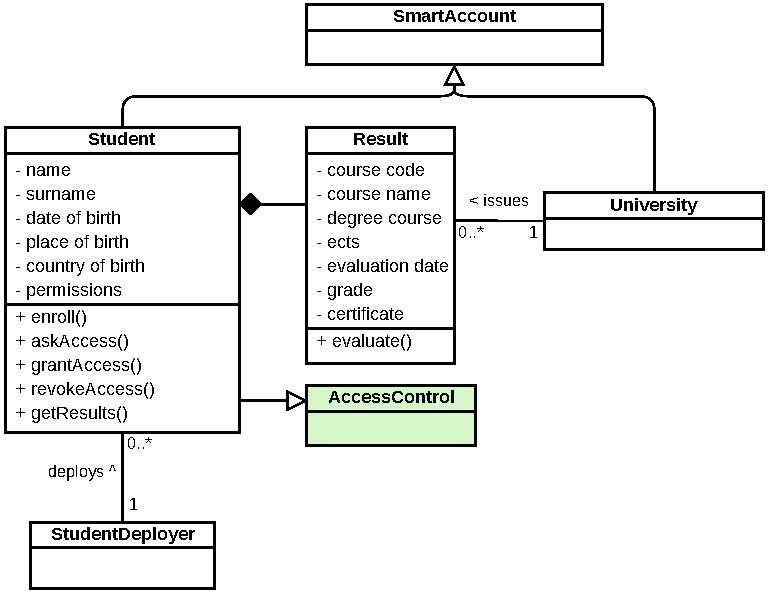
\includegraphics[width=0.7\textwidth]{figures/Student class diagram.pdf}
  \caption[Class diagram focused on \textit{Student} contract]{Class diagram showing a focused view of the \textit{Student} contract and its associated interactions. This view is a subset of the broader system architecture.}
  \label{fig:studentContractClass}
\end{figure}

\subsection{Deployment and Interaction Flow}
As illustrated in \cref{fig:useCaseCli} and \cref{fig:studentContractClass}, Student contracts are deployed by the StudentDeployer, which is invoked by the StudentsRegister contract when a university registers a new student in the \acrshort{ew} system. Delegating students registration to universities decentralizes the validation process: since universities already verify applications during their standard admissions procedures, they supply authenticated data directly to the system, thereby avoiding centralization and reducing administrative overhead. Relying solely on a central administrator to register both universities and potentially tens of thousands of students would be impractical.

Upon registration, the initiating university is automatically granted write permissions for the student's academic record, reflecting its role as the enrolling institution responsible for issuing evaluations. All subsequent interactions with the Student contract are carried out either by the browser extension or the \acrshort{sdk}. The browser extension is responsible for retrieving personal and academic data and managing permissions on the student's behalf. The \acrshort{sdk}, on the other hand, acts on behalf of universities to access and modify the student's academic wallet. To facilitate these interactions, the Student contract defines several structured data types, which are used for functions inputs and outputs. These structures improve code readability and usability by grouping related data into cohesive types. Instead of requiring users to  pass multiple separate parameters in a specific order, an approach that increases the risk of errors, developers can simply import the relevant structure and populate its fields. The data types defined in the Student contract are:

\begin{itemize}
    \item \textbf{EnrollmentInfo}: Contains the information required to enrol a student in a course; used as input for the enrolment function.
    \item \textbf{EvaluationInfo}: Contains the data needed to record an evaluation; used as input for the evaluation function.
    \item \textbf{Result}: Previously presented, this structure stores the details of a course attended by the student and is used to return the student's academic records.
    \item \textbf{StudentBasicInfo}: Represents the student's personal information.
    \item \textbf{StudentInfo}: A composite structure that includes StudentBasicInfo and a list of Result structures, representing the student’s complete academic profile.
\end{itemize}

\subsection{Vulnerabilities and Scalability}
This design is suitable not only for the testing environment but also for deployment in a real-world platform. In Solidity, the usage of aggregated data types, such as arrays or mappings, entails a gas cost that increases with the size of the data structure, particularly when looping or enumerate its content. However, in the context of a student's academic career, the number of universities requiring access to their academic wallet is typically limited, likely fewer than ten. As a result, the size of the permissions data structures remain small and the associated gas cost does not increase to a level that would pose significant issue.

A more significant concern arises with the storage of student's academic results, which are currently stored together in a single array. Recording a new evaluation for an existing course requires iterating through the array to locate the appropriate entry. If a student's results set grows to several tens of entries, this operation can incur high costs, undermining platform usability. To mitigate this issue, future enchantments can preserve the existing results array, allowing all records to be retrieved in a single transaction, while also maintaining a secondary mapping from the composite key (university address, course code) to the index of the corresponding result in the array. Although this mapping introduces a slight increase in the storage consumption, it enables constant-time lookups and updates for specific courses. This significantly lowers the gas cost for evaluations.  

Moreover, to minimize the overall cost of the \acrlong{ew} system and its operational expenses, all functions that do not modify the on-chain state, i.e., those that perform only data retrieval, are implemented as read-only operations. In Solidity, these are marked with the \textit{view} or \textit{pure} modifier and execute without gas cost. Given that read operations are generally more frequent that writes, this design choice further curtails the system's cumulative gas expenditures.

%%%%%%%%%%%%%%%%%%%%%%%%%%%%%%%%%%%%%%%%%%%%%%%%%%%%%%%%%%%%%%%%%%
% UNIVERSITY
%%%%%%%%%%%%%%%%%%%%%%%%%%%%%%%%%%%%%%%%%%%%%%%%%%%%%%%%%%%%%%%%%%
\section{University}
Since the primary focus of this work is on the interaction between students and their academic records, as well as the ownership of such data, the institutional accounts (\acrlong{sca}) of universities, implemented through the \textit{University} contract, are designed to be simpler that those of students, as illustrated in \cref{fig:universityContractClass}. Similar to the Student contract, the University contract extends the SmartAccount contract, enabling it to function as a \acrshort{sca} compatible with the account abstraction specification. As a result, universities can use their institutional wallet, via the \acrshort{sdk}, to perform blockchain transactions, which are then sponsored by the Paymaster (see \cref{sec:paymasterDesign}). 
\begin{figure}
  \centering
  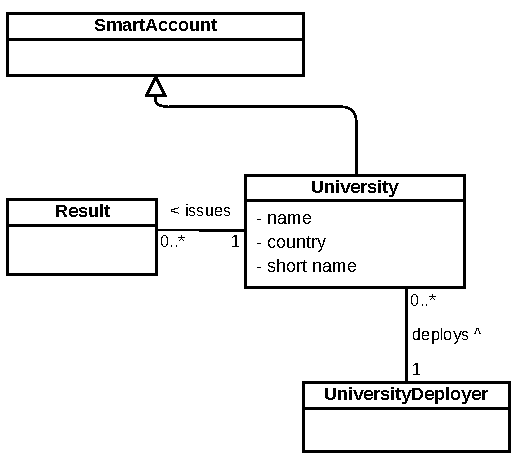
\includegraphics[width=0.4\textwidth]{figures/University class diagram.pdf}
  \caption[Class diagram focused on \textit{University} contract]{Class diagram showing a focused view of the \textit{University} contract and its associated interactions. This view is a subset of the broader system architecture.}
  \label{fig:universityContractClass}
\end{figure}

In addition, because universities are identified solely by their contract address in interactions with other smart contracts, the University contract also stores descriptive metadata, including the institution's name, country, and a short identifier. Apart from the UniversityDeployer, which is responsible for deploying the contract, the only components that interact directly with the University contract are the \acrshort{sdk} and the browser extension. When these components need to access university-related information, they do so using the institution's contract address. For instance, when a student retrieves their academic records, each record references the issuing university by it address. The browser extension must then query the blockchain to access the corresponding University contract and extract the relevant metadata. All such metadata functions are implemented as read-only calls, enabling gass-free data retrieval.   

%%%%%%%%%%%%%%%%%%%%%%%%%%%%%%%%%%%%%%%%%%%%%%%%%%%%%%%%%%%%%%%%%%
% STUDENT AND UNIVERSITY DEPLOYERS
%%%%%%%%%%%%%%%%%%%%%%%%%%%%%%%%%%%%%%%%%%%%%%%%%%%%%%%%%%%%%%%%%%
\section{StudentDeployer and UniversityDeployer}
The deployment of Student and University contracts, corresponding to \textit{FR 5} and \textit{FR 2} in \cref{tab:funcReq} respectively, is handled by the \textit{StudentDeployer} and \textit{UniversityDeployer} contracts, as depicted in \cref{fig:deployersContractClass}. When a system administrator registers a new university, or a university registers a new student through the \acrshort{sdk}, they interact with the StudentsRegister smart contract. This contract, in turn, invokes one of the deployer contracts to create the corresponding smart contract instance. This architecture implements the factory pattern, a design principle commonly used in object-oriented programming to abstract the creation of objects. In the context of the \acrshort{ew} system, the deployer contracts abstract and encapsulate the instantiation of new Student and University contracts.

The adoption of the factory pattern offers several advantages over embedding the deployment logic directly within the StudentsRegister contract:
\begin{itemize}
    \item It separates the contract creation logic from the registration logic, improving modularity and maintainability.
    \item It reduces the complexity of the StudentsRegister contract by externalizing the deployment process.
    \item It minimizes the contract size of StudentsRegister. In Solidity, deploying a contract via the \textit{new} keyword requires embedding the bytecode of the deployed contract, which increases the size of the calling contract. Since Solidity enforces a maximum contract size of 24576 bytes, including large deployment code directly could exceed this limit. Using external deployer contracts bypass this issue.
\end{itemize}

\begin{figure}
  \centering
  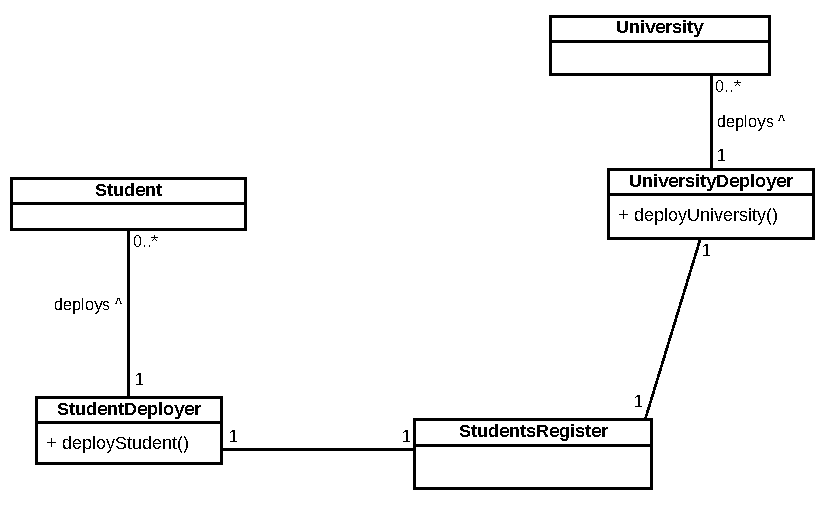
\includegraphics[width=0.7\textwidth]{figures/Deployers class diagram.pdf}
  \caption[Class diagram focused on \textit{StudentDeployer} and \textit{UniversityDeployer} contracts]{Class diagram showing a focused view of the \textit{StudentDeployer} and \textit{UniversityDeployer} contracts and their associated interactions. This view is a subset of the broader system architecture.}
  \label{fig:deployersContractClass}
\end{figure}

The decision to centralize deployments through the StudentsRegister contract was also motivated by gas efficiency. On blockchain platforms, reducing the number of transactions typically leads to lower gas costs. By combining the deployment of a contract and the registration of its address into a single transaction, the system reduces the overall gas consumption required for onboarding new entities.

%%%%%%%%%%%%%%%%%%%%%%%%%%%%%%%%%%%%%%%%%%%%%%%%%%%%%%%%%%%%%%%%%%
% STUDENTS REGISTER
%%%%%%%%%%%%%%%%%%%%%%%%%%%%%%%%%%%%%%%%%%%%%%%%%%%%%%%%%%%%%%%%%%
\section{StudentsRegister}
This section presents the \textit{StudentsRegister} smart contract, which functions as the \acrlong{ew} ledger. It stores the addresses of all student and university academic wallets and links them to their respective \acrlong{eth} wallets. This contract is deployed by the system administrator, who thereby becomes its owner and gains access to the functionalities restricted through the Ownable library contract. The Ownable contract, provided by the OpenZeppelin library, establishes an ownership model where certain functions are accessible only to the contract's owner. It also enables ownership transfer to another \acrshort{eth} wallet or smart contract, if needed.
During deployment, the StudentsRegister contract requires the addresses of the already deployed StudentDeployer and UniversityDeployer contracts, which it must invoke to create new smart accounts. Additionally it must be configured with the address of the EntryPoint contract responsible for enabling account abstraction.
\begin{figure}
  \centering
  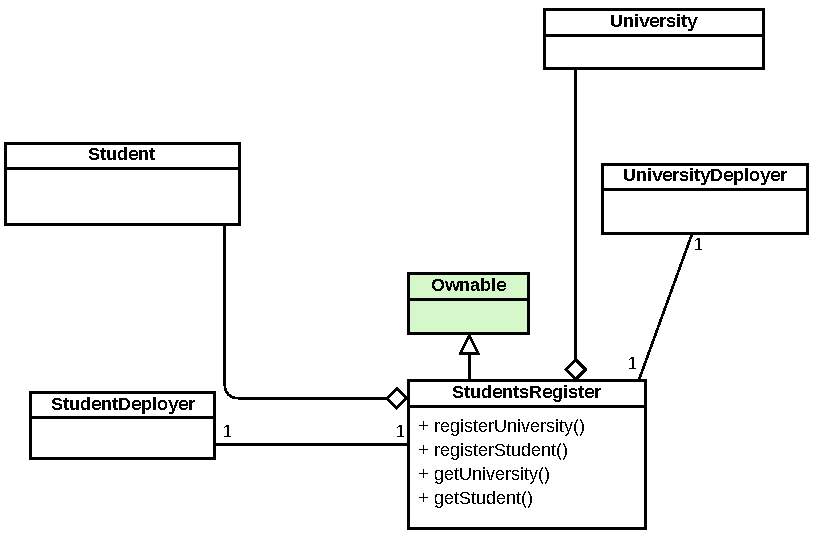
\includegraphics[width=0.7\textwidth]{figures/StudentsRegister class diagram.pdf}
  \caption[Class diagram focused on \textit{StudentsRegister} contract]{Class diagram showing a focused view of the \textit{StudentsRegister} contract and its associated interactions. This view is a subset of the broader system architecture.}
  \label{fig:studentsRegisterContractClass}
\end{figure}

\subsection{Core Functionalities}
As illustrated in \cref{fig:studentsRegisterContractClass}, the StudentsRegister contract provides five core functionalities:

\begin{enumerate}
    \item \textbf{Register a new university}: This function allows the system administrator (i.e., the contract owner) to register a new university within the \acrshort{ew} system by submitting its institutional information, name, country, a short identifier, and its \acrlong{eth} wallet address. The wallet address is stored within the StudentsRegister contract and also utilized in the corresponding University contract to define account ownership. This functionality fulfils requirement \textit{FR 1} in \cref{tab:funcReq}. To prevent duplicate entries, the function checks whether the university's \acrlong{eth} wallet address is already present in the registry. Upon successful validation, the StudentsRegister contract invokes the UniversityDeployer contract to instantiate the university’s smart account and stores the resulting address alongside the provided wallet address. Access to this function is restricted to the contract owner to ensure that only verified and authorized institutions can be registered.

    \item \textbf{Retrieve a university smart account address}: This function allows a university to obtain the address of its \acrshort{sca} by referencing its \acrshort{eoa} address. This functionality supports \textit{FR 3} in \cref{tab:funcReq} and is integrated into the \acrshort{sdk}, which uses the university's \acrlong{eth} wallet for authentication and retrieves the corresponding smart account address to enable operations under the account abstraction model. As a read-only operation, it incurs in no gas cost.
    
    \item \textbf{Register a new student}: This function, restricted to validated universities, allows them to register a new student by providing the student's \acrlong{eth} wallet address along with relevant personal details. To prevent duplicate registrations, the function verifies whether the student's \acrshort{eth} wallet is already present in the system. This operation fulfils requirement \textit{FR 4} in \cref{tab:funcReq}. The wallet address is recorded in the StudentsRegister contract and referenced in the associated Student contract to establish ownership. Universities invoke this functionality through the \acrshort{sdk}, as with all other smart contract interactions.
    
    \item \textbf{Retrieve a student smart account address}: This function enables a student to retrieve the address of their smart account using their \acrlong{eth} wallet address. It is primarily used during the login process handled by the browser extension, addressing requirement \textit{FR 10} in \cref{tab:funcReq}. When a student logs in using their ID and password, the extension derives the corresponding \acrlong{eth} wallet and queries the StudentsRegister contract to retrieve the associated smart account address. If a valid address is returned, the authentication process is considered successful. As this function does not alter any state on the blockchain, it is implemented as a view function to leverage gas-free execution.
\end{enumerate}

\subsection{Scalability and Gas Considerations}
In contrast to the Student contract, StudentsRegister is designed to mitigate unbounded gas cost associated with growing dynamically growing data structures. It stores student and university addresses in mappings, which provide direct, constant-time access by key. Since the system does not require iteration over all entries during standard transaction execution, the gas cost of insertion operations remains stable and independent of the total number of registered entities. This architectural choice ensures that the registry can scale efficiently without incurring increasing gas fees.

%%%%%%%%%%%%%%%%%%%%%%%%%%%%%%%%%%%%%%%%%%%%%%%%%%%%%%%%%%%%%%%%%%
% PAYMASTER
%%%%%%%%%%%%%%%%%%%%%%%%%%%%%%%%%%%%%%%%%%%%%%%%%%%%%%%%%%%%%%%%%%
\section{Paymaster}
\label{sec:paymasterDesign}
One of the system's key feature is that blockchain usage is nearly transparent for users. Students do not directly interact with wallets or perform transactions themselves, and universities only need the private key associated with their \acrshort{eoa} to manage their institutional smart wallet. This level of abstraction is made possible by the \textit{Paymaster}, a smart contract deployed on the blockchain that sponsors all transactions made by users. This design directly readdressing \textit{NFR 5} (see \cref{tab:nonFuncReq}), which emphasizes minimizing the complexity of interactions with the system for end users.

Without the Paymaster, the system would require a mechanism to fund user wallets, presenting three primary options:

\begin{enumerate}
    \item Each user funds their own wallet.
    \item Universities fund the wallets of both students and themselves.
    \item The \acrshort{ew} system centrally manages and funds all wallets.
\end{enumerate}
Each approach has significant drawbacks. The first and second require users to manage cryptocurrency wallets and purchase tokens, which increases complexity and cost, especially burdensome for students. The third alternative still introduces administrative overhead and security concerns related to managing a large number of wallets.

\begin{figure}
  \centering
  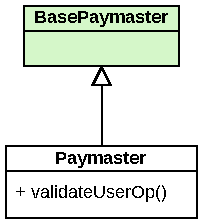
\includegraphics[width=0.2\textwidth]{figures/Paymaster class diagram.pdf}
  \caption[Class diagram focused on \textit{Paymaster} contract]{Class diagram showing a focused view of the \textit{Paymaster} contract. This view is a subset of the broader system architecture.}
  \label{fig:paymasterContractClass}
\end{figure}
Our solution utilizes a Paymaster that, as shown in \cref{fig:paymasterContractClass}, implements the BasePaymaster abstract contract, developed as part of ERC-4337. For simplicity, our current implementation sponsors all user operations (transactions) it receives, without validating their origin or gas cost. The only enforced constraint, inherited from BasePaymaster, is that transactions must be routed through a known EntryPoint contract.
This configuration is suitable for testing environments such as local or test networks, where there is no risk of losing real tokens. In a real-world deployment, a more robust implementation would be necessary, specifically, one that integrates with the StudentsRegister contract to verify that the transaction sender is a verified student or university. 